\chapter{Introducción}


\section{Normatividad escolar y su importancia}

Como seres sociales, existe la necesidad de establecer acuerdos que regulen el comportamiento y las formas de crear relaciones con otros individuos. Estos acuerdos son de suma importancia para facilitar interacciones y las actividades de organizaciones sociales. En algunas ocasiones estos acuerdos mutuos entre individuos llegan a cuestionarse por causas de conflictos de principios. Un estudio ha delimitado tres dominios sobre los cuáles los valores se construyen \parencite{thornberg}:

\begin{itemize}
    \item \textbf{moral}: conceptos de bienestar humano, justicia y verdad.
    \item \textbf{convencional}: conceptos éticos basados en autoridad, tradiciones, consensos y acuerdos.
    \item \textbf{personal}: conceptos que pertenecen principalmente al comportamiento de uno mismo basado en preferencias y decisiones que buscan la mayor satisfacción posible.
\end{itemize}

Esto nos lleva a buscar una referencia en común que se vuelve necesaria para un orden, ya que si no se establecen conceptos uniformes la forma de evaluar el comportamiento se vuelve ambiguo. Se debe tener en alta estima o el respeto hacia un autoridad en común cuando se tratan de valores convencionales. Estas convenciones deben ser vistas como parte de un sistema fijo y requieren adherencia mutua entre individuos \parencite{turiel}.

Mientras que los dominios morales y personales quedan abstraídos en la subjetividad, el dominio convencional se establece bajo la autoridad y uniformidad de comportamiento mediante un \textit{convenios sociales} o \textit{contrato social} que optimiza la integración de todos los individuos de la mejor manera posible. Esto es posible mediante normas que se fundamentan de manera oficial como resultado de este acuerdo con el uso de autoridad. Mediante un sistema de este tipo se puede trasladar este objetivo a los distintos grupos que la sociedad forma para cumplir diferentes funciones.

Para poder enunciar de manera oficial estas bases, se necesitan leyes y reglamentos. Una \textbf{ley} es una norma emitida establecida de manera jurídica por un estado a través de sus poder legislativo del Estado, junto con las consecuencias de la infracción de tales leyes \parencite{davidrogers}. Sin embargo, la ley no da especificación a detalle de lo que consiste el cumplimiento, Son los \textbf{reglamentos} determina los procesos y definiciones a detalle para complementar el efecto jurídico de las normas. 

Un \textbf{marco jurídico} es el conjunto de leyes y normas que forman la base legal. En ella se determinan las formas de organización y funciones de una sociedad. El ejercicio de los marcos jurídicos es sumamente importante para garantizar que se cumplan los derechos que le corresponden a un conjunto de individuos para regular la forma en que se relacionan. Dentro de cualquier ámbito, se debe establecer una autoridad que emita y se encargue de hacer cumplir ciertas normas para que el orden se mantenga de manera óptima para todos.

Un \textbf{marco normativo} son las disposiciones legales que regulan asuntos específicos de los procesos para el funcionamiento de esa sociedad. Es decir, las diversas organizaciones establecen un marco normativo para que una autoridad pueda regular las actividades de las diversas materias que le competen. \textit{El marco jurídico da la base legal para que establezcan las reglas específicas para atender a los procesos esenciales de una organización mediante el marco normativo}.

Ambos conceptos se reducen a la definición de los derechos y obligaciones que un individuo tiene como integrante de una organización y las implicaciones que consisten en su participación. Es por ello que como sociedad se divulgue y se haga del conocimiento a la comunidad interesada. Esto se hace a través de establecer leyes y reglamentos en un \textbf{documento legal}. En México, las leyes y reglamentos se organizan de manera estructural, la cual se debe dividir de acuerdo a la extensión de asuntos que trata un mismo reglamento \parencite{lopezruiz}. Estas divisiones estructurales son las siguientes:

\begin{enumerate}
    \item \textbf{Libros}: recopilan leyes muy extensas que se pueden dividir por su complejidad.
    \item \textbf{Títulos}: utilizado en leyes extensas, esta agrupación divide partes claramente diferenciadas.
    \item \textbf{Capítulos}: tiene un contenido unitario que no es fijado solo con base en el número de artículos sino que dependen de la materia que tratan.
    \item \textbf{Secciones}: utilizado cuando la materia es extensa y requiere subdividir a los artículos, pero no es suficiente para ser tratado como capítulo.
    \item \textbf{Artículos}: unidad normativa que regula un tema o precepto que se dicta de forma de un solo enunciado.
    \item \textbf{Párrafos}: unidad parcial de un artículo que divide la redacción.
    \item \textbf{Apartados}: Utilizado de manera poco común, funciona para dividir todo lo referente a la misma materia normativa. Se deben diferenciar con letras mayúsculas.
    \item \textbf{Fracciones}: Enumeran una serie de atribuciones, requisitos, obligaciones, etc, otorgados en un artículo. Se separan con números romanos.
    \item \textbf{Incisos}: División mínima legal utilizada para enumerar elementos o lista de objetos y entidades como componentes de la misma norma. Se numeran con letras minúsculas cerradas por medio de paréntesis de cierre, sin punto ni guión.
\end{enumerate}

Siendo la estructura temática un aspecto esencial de la ley, se debe resaltar que son los \textbf{artículos} la división elemental y fundamental de las leyes que constituye una disposición atómica. Esta misma estructura aplica a asuntos internos de diversas instituciones, que requieren establecer sus normas para que sus integrantes se adhieran en todo momento para cumplir con las finalidades establecidas.


\subsection{Marco Normativo del Instituto Politécnico Nacional}
\label{subsec:marco-normativo-ipn}

El Instituto Politécnico Nacional se rige por su propia Ley Orgánica y se encuentra capaz de expedir los acuerdos en los que se dictan los reglamentos necesarios para el cumplimiento de los objetivos académicos y supervisar que los procesos incluidos en el marco normativo sean apegados a los mismos reglamentos para regular la vida social y el desarrollo profesional de sus integrantes.

El artículo 3 de la Constitución Política de los Estados Unidos Mexicanos dicta que:

\begin{quote}
    \textit{La educación se basará en el respeto irrestricto de la dignidad de las personas, con un enfoque de derechos humanos y de igualdad sustantiva. Tenderá a desarrollar armónicamente todas las facultades del ser humano y fomentará en él, a la vez, el amor a la Patria, el respeto a todos los derechos, las libertades, la cultura de paz y la conciencia de la solidaridad internacional, en la independencia y en la justicia; promoverá la honestidad, los valores y la mejora continua del proceso de enseñanza aprendizaje.}
\end{quote}

Es este principio el que da la base para que las actividades desarrolladas por el Instituto Politécnico tengan un sentido social humano equitativo para todos sus integrantes en beneficio del país. Actualmente existen 29 reglamentos. Estos reglamentos derivan a cada dependencia del instituto, incluyendo a la Escuela Superior de Cómputo (ESCOM). El marco normativo de la ESCOM completamente de las disposiciones emitidas por el Instituto Politécnico Nacional, que a su vez se le considera como un \textit{órgano desconcentrado de la Secretaría de Seguridad Pública, cuya orientación general corresponde al Estado}, de acuerdo con el artículo 2 de la Ley Orgánica del Instituto Politécnico Nacional.


De esta manera, la ESCOM participa en el ejercicio de un sistema de normas que ayudan a establecer procesos y reglamentos que exigen el cumplimiento de obligaciones, pero usando su derecho en todo momento cuando su comunidad académica realiza las actividades cotidianas correspondientes a sus funciones. Como por ejemplo, la forma en cómo se regulan las opciones de titulación quedan establecidas en el \textit{Reglamento de Titulación Profesional}. El marco normativo también da vigencia a las autoridades escolares mediante la \textit{Ley Orgánica}.

\subsection{La importancia de la divulgación}

Todo integrante de esta comunidad de la Escuela Superior de Cómputo queda implicado en la práctica de las normas en todo momento. Por lo tanto, el marco normativo debe ser referencia y se debe hacer de su conocimiento. 

\begin{figure}
    \centering
    
\includegraphics[scale=0.225]{images/1/pagina-normatividad.png}
    \caption{Captura de pantalla del sitio con el contenido referente al marco normativo del IPN.}
    \label{fig:sitio-normatividad}
\end{figure}

Los recursos que conforman parte de este marco normativo se pueden encontrar dentro del sitio \url{https://www.ipn.mx/normatividad/}. La figura \ref{fig:sitio-normatividad} muestra una captura de pantalla de este sitio que contiene categorías distintas para la ubicación de documentos emitidos por el Instituto Politécnico Nacional; estas categorías son: \textit{lineamientos}, \textit{guías normativas}, \textit{reglamentos}, \textit{normatividad abrogada}, \textit{avisos}, \textit{manuales}, y \textit{programas institucionales}.

La aplicación y supervisión de los reglamentos es igualado por la importancia de la divulgación de los mismos para que sea justificado. Esta correlación de conocimiento-aplicación queda en su comunidad como parte de su deber civil para garantizar integridad las funciones que desempeñan.

Teniendo eso en mente, toda actividad efectuada por los integrantes de la Escuela Superior de Cómputo se apegará a su Ley Orgánica y al marco normativo en general. Esto envuelve múltiples aspectos de la vida social de los que integran la comunidad académica del instituto y las acciones cotidianas que desempeñan para la formación profesional.

Algunos ejemplos de estos aspectos cotidianos son:

\begin{itemize}
    \item \textbf{Organización del instituto}: estructura de las unidades académicas y administrativas que requiere el instituto para ejercer sus funciones.
    \item \textbf{Trayectoria académica}: definición de procesos y establecimiento de derechos y obligaciones al que el alumnado deberá apegarse.
    \item \textbf{Opciones de titulación}: cuáles son, en qué consisten y los requerimientos para acreditar el derecho a la titulación.
\end{itemize},

\section{Planteamiento del Problema}

Una vez que se considera los recursos y su accesibilidad, también se debe tomar en cuenta los problemas inherentes a la información. Hemos establecido la importancia de la relación conocimiento-aplicación, sin embargo la consulta misma de los reglamentos trae consigo diversos obstáculos.

Uno de ellos es la \textbf{sobrecarga de información}, que es un problema común que una persona puede enfrentarse al contar con mas conocimiento de la que puede asimilar naturalmente. Un estudio demuestra que demasiada información tiende a provocar un desinterés, confusión y frustración en lugar de aceptarla. \parencite{jinwonrong}. 

La cantidad de elementos a conocer se dispersa al considerar la cantidad de materias distintas tratadas en el marco normativo, la cantidad de documentos que existen para tratarla y cuántos artículos cuenta cada uno de esos documentos. Entre mayor sea la cantidad de elementos que conforman este marco normativo, mayor será la dispersión de esta búsqueda.
s
Por ejemplo, el apartado de \textbf{Reglamentos} mostrados en el sitio de normatividad (figura \ref{fig:sitio-normatividad}) cuenta con \textbf{52 documentos en total}:
\begin{itemize}
    \item 2 Códigos
    \item 21 Acuerdos
    \item 29 Reglamentos
\end{itemize}

Los 29 reglamentos son el lugar de interés para la investigación normativa. Para que una persona pueda tener un manejo suficiente de estos recursos, esta persona deberá conocer (o en su defecto investigar):

\begin{itemize}
    \item la materia normativa a la que se refiere cada documento
    \item cuáles de ellos involucran el concepto a buscar
    \item en qué partes del documento se habla de ese concepto
\end{itemize}

Si, por ejemplo, se desea buscar artículos que hablen de la titulación, podría deducir en cuáles reglamentos es mas probable que esté y hacer una búsqueda obteniendo resultados que indiquen que se encontró algo en los siguientes documentos: Reglamento Interno, Reglamento de Titulación y Reglamento General de Estudios.

Pero cada documento abarcaría asuntos distintos relacionados al mismo concepto. Por ejemplo, en el Reglamento Interno encontraremos artículos que establecen el derecho a la titulación mediante el cumplimiento de algunos requisitos, mientras que en e Reglamento de Titulación se establecen las modalidades y sus respectivos requisitos.

También existe el problema de búsquedas exactas para conceptos similares relacionados. Por ejemplo cuando se desea obtener los artículos que se refieran a los hechos delictivos, pero la búsqueda se hace mediante  un concepto similar \textit{crimen}, \textit{delito}, \textit{infracción}, etc. Un usuario que desconozca el vocabulario formal no sabrá con cuál de estos términos hacer la búsqueda exacta.

. \textbf{¿Cómo podría consultarse los artículos de manera que se busquen los que cumplan esa relación de conceptos?}

\section{Objetivo}

Desarrollar un chatbot que pueda orientar a la comunidad de ESCOM de sus derechos y obligaciones dentro
del marco normativo establecido por los reglamentos del Instituto Politécnico Nacional.

La orientación normativa escolar se obtendrá de los siguientes documentos:

\begin{itemize}
    \item Ley Orgánica del Instituto Politécnico Nacional,
    \item Reglamento Interno del Instituto Politécnico Nacional,
    \item Reglamento General de Estudios del Instituto Politécnico Nacional, y
    \item Reglamento de Titulación Profesional del Instituto Politécnico Nacional
\end{itemize}

\section{Justificación}

La motivación principal de este proyecto es el hecho de que hasta la fecha no existen herramientas que cumplan el objetivo de facilitar la consulta en los documentos anteriormente nombrados. Como ya se vio en la problemática, para realizar una consulta de información en especifico, se requiere de tiempo y de una terminología, que muy probablemente se desconoce.

Con la transformación de la información a medios digitales, la accesibilidad al conocimiento puede facilitarse a una comunidad a través de la tecnología. De aquí surge la oportunidad de implementar sistemas de \textbf{recuperación de información} automatizados mediante el desarrollo de software. Hoy en día esto es posible gracias al desarrollo de sistemas de recuperación de información digital, los cuáles han sido tomados para la mejora de la accesibilidad a la información en todas sus representaciones.

\section{¿Qué es un chatbot?}

% Sugiero el siguiente order:
% 2. Usos anteriores  tiene y ejemplos de exito
% 3. Describir el por que seria bueno en el desarrollo y compar con otro tipo de sistemas

Cuando se trata de una asesoría, una persona tiende a querer expresar una duda a una persona que brinda apoyo para despejarla. La persona se vuelve un interfaz entre la persona y el conocimiento y cumple una función de orientación. Este proceso de \textit{expresar duda} y \textit{obtener orientación} es precisamente el proceso que se pretende automatizar en un \textbf{chatbot}.

¿Qué es un chatbot? Como lo indica su nombre en inglés, es un software que simula \textit{hablar} o comunicarse. Es un software que proporciona un servicio a través de una conversación, intentando emular la inteligencia humana para responder adecuadamente. Es por esto que también se le conocen como \textbf{agentes virtuales}. Se busca poder aprovechar la oportunidad de asistir a usuarios a realizar procesos que generalmente requiere de la comunicación de una persona que requiere un servicio con otra persona que lo ofrece.

Es por ello que se tienden a utilizar en procesos de atención a clientes o al público en general; pedir una pizza, agendar un vuelo, reservar una habitación en un hotel, etc. Al igual que poder ser atendido en persona para realizar alguno de estos servicios, empresas han visto la oportunidad de automatizar este proceso de atención delegándosela a un chatbot a a través de sitios de internet, aplicaciones en el celular e incluso redes sociales. Por ejemplo, BBVA desarrollo un asistente virtual para realizar operaciones bancarias mediante una conversación textual o hablada.

\begin{figure}[ht]
    \centering
    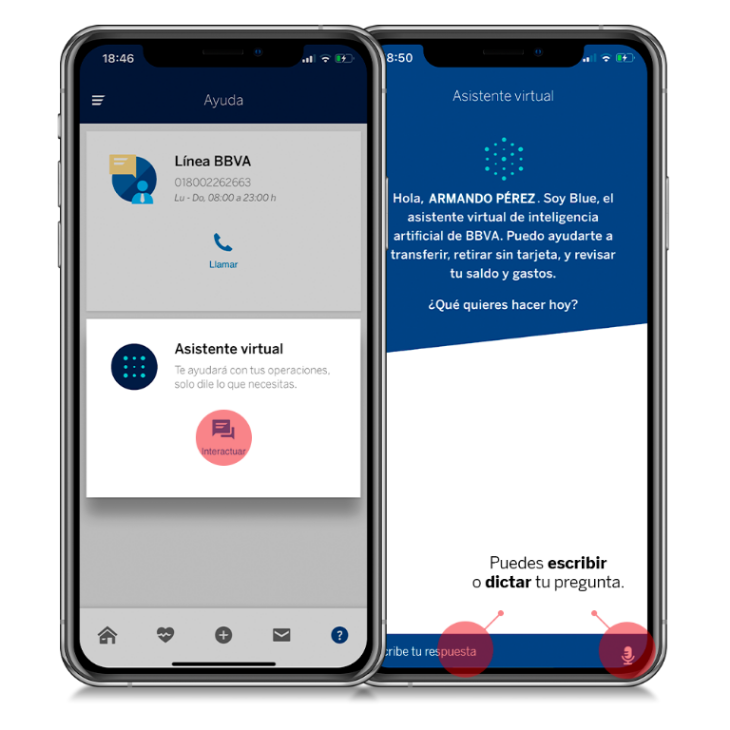
\includegraphics[scale=0.375]{images/1/blue-bbva}
    \caption{Asistente virtual Blue.Fuente: \url{https://www.bbva.com/es/mx/cuatro-funcionalidades-de-blue-para-facilitar-la-vida-de-los-clientes/}}
    \label{fig:blue-bbva}
\end{figure}

Un reporte hecho por la empresa \textit{Reports and Data} estima que la demanda de los chatbots tenga un crecimiento de 30.9\% en el 2026 en comparación a la demanda del año 2019 (figura \ref{fig:demanda-chatbots}) . Esto es porque muchas empresas e instituciones buscan formas de inovar el contacto y divulgación de información a través de un asistente virtual, \textit{queriendo volver obsoleto al modelo actual} de navegación de sitios web como una interfaz a la información; \textbf{es mas factible interactuar con información mediante los chatbots}.

\begin{figure}[ht]
    \centering
    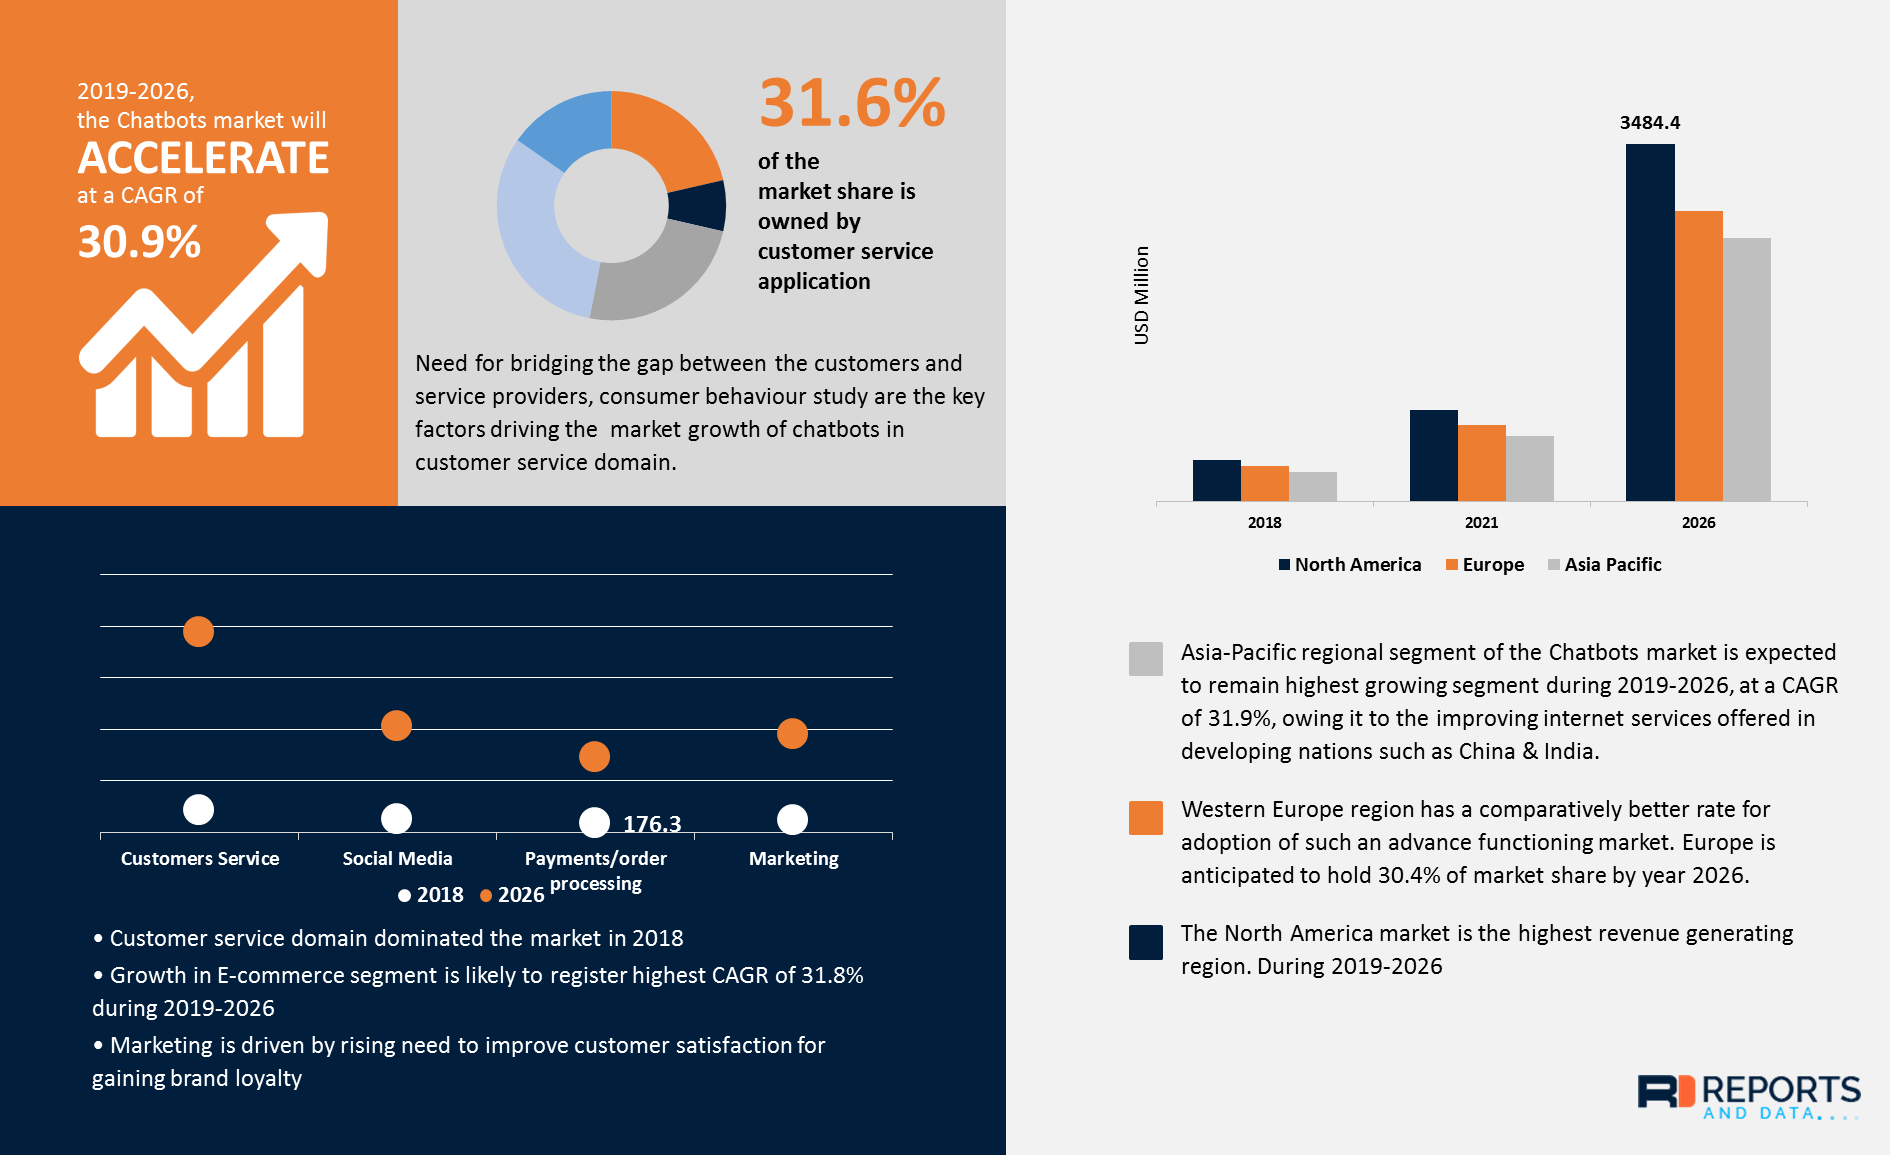
\includegraphics[scale=0.5]{images/1/demanda-chatbots}
    \caption{Fuente: \url{https://www.reportsanddata.com/report-detail/chatbot-market}}
    \label{fig:demanda-chatbots}
\end{figure}

\section{El Uso de un Chatbot Para Orientación Normativa}

\begin{figure}[ht]
    \centering
    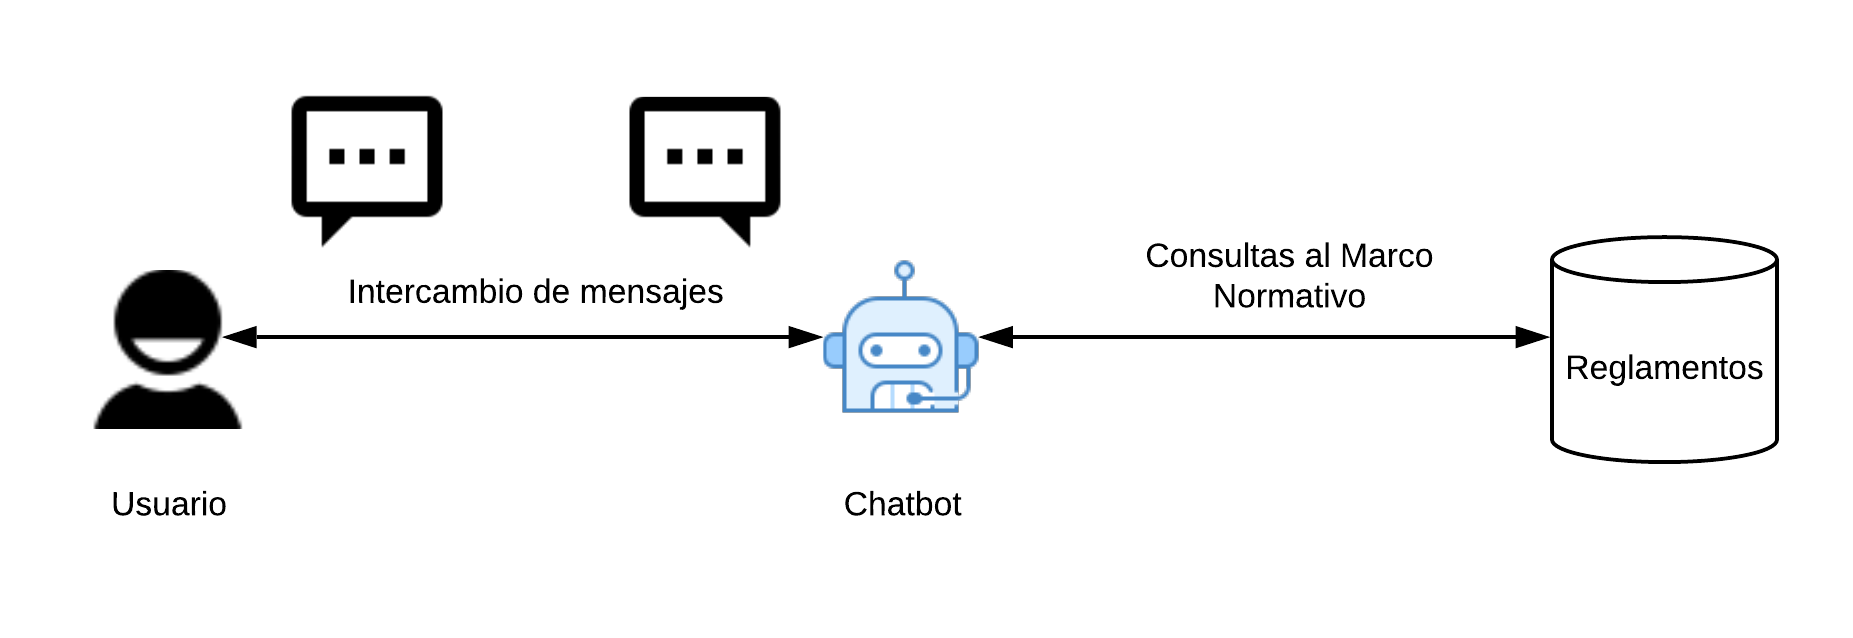
\includegraphics[scale=1]{images/1/propuesta-aplicacion.png}
    \caption{Automatización de una asesoría mediante un chatbot}
    \label{fig:propuesta-aplicacion}
\end{figure}

¿Por qué un chatbot? Una alternativa en la que se podría implementar una solución basada en crear un \textbf{motor de búsqueda}. Esta alternativa podría tener un desarrollo mas sencillo, pero a costo de una interfaz con mas elementos de configuración para el tipo de búsqueda. La compensación de complejidad de desarrollo por una mayor experiencia de usuario mediante el intercambio de dialogo es la principal motivación para decidir implementar la solución mediante un chatbot, ya que un buen diseño conversacional elimina la necesidad de que un usuario configure entradas y parámetros antes de utilizarlo.

Por naturaleza, somos capaces de utilizar el fenómeno de la comunicación para intercambiar información múltiples maneras con el mismo significado, o si no algo similar. En este proyecto aprovecharemos la facilidad de la expresión de diálogo y con ello establecer funcionalidades para cumplir el objetivo propuesto. Contrario a esto, sería que el usuario introduzca de manera rígida de un formulario o la introducción de parámetros de búsqueda.

% Move this to proposal
Adicional a esto, la integración de estos servicios a los portales web del Instituto Politécnico Nacional podrían aprovechar el uso de canales de comunicación. Esto para auxiliar a la comunidad escolar en la obtención de una asesoría previa a la intervención de una persona experta en el tema.
% Intetrate to current communication channels

Este proyecto propone el desarrollo de un chatbot que funcione como sistema de recuperación de información para atender los problemas mencionados. Estará disponible a través de una aplicación web que se pueda utilizar desde un navegador web que funcionará como cliente de este servicio.
